


\chapter{Misurazione della Superficie di Fermi}

Ci sono diversi effetti sperimentali che permettono di misurare la superficie di Fermi; una volta nota la sua forma, è possibile ricavare informazioni approfondite sulla struttura delle bande elettroniche nel solido.

\section{De Haas--van Alphen Effect}

L'effetto De Haas--van Alphen consiste nella misurazione della magnetizzazione \(M\) di un campione (ad esempio, di Bismuto) in funzione del campo magnetico \(H\) a temperature molto basse (ad esempio, \SI{14.2}{\kelvin}).  \\
In tali esperimenti si osservano oscillazioni del rapporto \(M/H\) nonché oscillazioni analoghe nelle grandezze come la suscettività magnetica, la conduttività e la magnetoresistenza, quando queste vengono tracciate in funzione dell'inverso del campo magnetico, \(1/H\).\\\\

Landau aveva già mostrato che l'oscillazione di un elettrone libero in campo magnetico deriva dalla quantizzazione delle orbite elettroniche.  
Successivamente, Osanger introdusse quella che viene chiamata la \textbf{legge di Osanger}, secondo la quale il cambiamento nell'inverso del campo magnetico in un singolo periodo d'oscillazione è dato da:
\[
\Delta\left(\frac{1}{H}\right) = \frac{2\pi e}{\hbar c}\,\frac{1}{A_e}\,,
\]
dove \(A_e\) \textbf{rappresenta l'area della sezione trasversale della superficie di Fermi}, calcolata lungo la direzione normale al campo magnetico.  
\textbf{Variando il campo magnetico, dunque, si possono attraversare sezioni diverse della superficie di Fermi e, in questo modo, si può “mappare” l'intera superficie.}  \\
Si ricorda che gli elettroni coinvolti sono quelli prossimi all'energia di Fermi, poiché solo loro partecipano attivamente alla conduzione.

\begin{figure}[H]
	\centering
	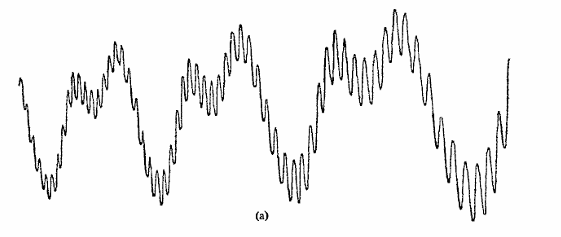
\includegraphics[width=0.8\textwidth]{images/6-Superficie-Fermi/vanalphen.png}
	\caption{Esempio di oscillazioni dell'effetto De Haas--van Alphen nel Renio.}
	\label{fig:vanalphen}
\end{figure}


\subsection{Origine del Fenomeno Oscillatorio}
Per comprendere a fondo il comportamento oscillatorio delle varie grandezze al variare del campo magnetico, è necessario analizzare come la presenza del campo alteri la densità degli stati elettronici.

\subsubsection{Livelli di Landau}

Per investigare la struttura degli stati quantizzati in campo magnetico, si risolve l'equazione di Schrödinger per una particella carica in presenza di un campo magnetico.  \\
Consideriamo elettroni confinati in una "box" di lato \(L\) e imponiamo il gauge di London con il campo magnetico \(H\) orientato lungo l'asse \(z\).  
Si adotta il gauge di Coulomb (London) tale che:
\[
\mathbf{H}=(0,0,H) \quad \text{e} \quad \mathbf{A}=(0,Hx,0),
\]
con la condizione \(\vec{\nabla} \cdot \mathbf{A}=0\).  
Passando agli operatori, il momento canonico si sostituisce con:
\[
\hat{\mathbf{p}} \to \hat{\mathbf{p}} - \frac{q}{c}\,\mathbf{A}\,,
\]
e considerando la carica elettronica \(q = -e\) (si usi la convenzione in cui \(c\) è posto uguale ad 1 se non diversamente indicato), si scrive:
\[
\hat{\mathbf{p}} \to \hat{\mathbf{p}} + \frac{e}{c}\,\mathbf{A}\,.
\]
L'hamiltoniana del sistema diventa quindi:
\[
\hat{\mathcal{H}} = \frac{1}{2m}\Bigl[\hat{p}_x^2 + \hat{p}_z^2 + \bigl(\hat{p}_y+eHx\bigr)^2\Bigr]\,.
\]
Espandendo il termine \(\bigl(\hat{p}_y+eHx\bigr)^2\) e raggruppando i termini, si ottiene:
\[
\hat{\mathcal{H}} = \frac{\hat{p}_z^2}{2m} + \frac{\hat{p}_y^2}{2m} + \omega_c\, \hat{p}_y + \frac{\hat{p}_x^2}{2m} + \frac{1}{2}m\omega_c^2\, x^2\,,
\]
dove la frequenza di ciclotrone è definita come:
\[
\omega_c = \frac{eH}{m}\,.
\]

Si ipotizza una soluzione del tipo:
\[
\psi(x,y,z)= C\,e^{ik_z z}\, e^{ik_y y}\, f(x)\,,
\]
con \(C\) costante di normalizzazione.  \\
Inserendo questa forma nell'equazione agli autovalori
\[
\hat{\mathcal{H}}\,\psi = \varepsilon\, \psi\,,
\]
si separa il problema nelle variabili \(z\) e \(y\) – che danno termine \(\frac{\hbar^2 k_z^2}{2m}\) e \(\frac{\hbar^2 k_y^2}{2m}+\hbar\,k_y\,\omega_c\,x\) – e nella variabile \(x\):
\[
\left[\frac{\hat{p}_x^2}{2m}+ \frac{1}{2}m\omega_c^2 x^2\right]\,f(x) + \left[\frac{\hbar^2 k_y^2}{2m}+ \hbar\,k_y\,\omega_c\,x\right]f(x) + \frac{\hbar^2 k_z^2}{2m}\, f(x) = \varepsilon\, f(x)\,.
\]
La parte in \(x\) può essere riarrangiata in maniera tale da completare il quadrato.  \\
Osserviamo che:
\[
\frac{\hbar^2 k_y^2}{2m} + \hbar\,k_y\,\omega_c\, x + \frac{1}{2}m\omega_c^2\, x^2
\]
può essere scritta riscrivendo il termine lineare in \(x\) in modo da completare il quadrato.  
Si definisce:
\[
x_0 = -\frac{\hbar k_y}{eH}\,,
\]
in modo da poter scrivere:
\[
\frac{\hbar^2 k_y^2}{2m} + \hbar\,k_y\,\omega_c\, x + \frac{1}{2}m\omega_c^2\, x^2 = \frac{1}{2}m\omega_c^2\,(x-x_0)^2\,.
\]
Pertanto, l'equazione per \(f(x)\) diventa quella dell'oscillatore armonico unidimensionale:
\[
\left[\frac{\hat{p}_x^2}{2m} + \frac{1}{2}m\omega_c^2\,(x-x_0)^2\right] f(x) = \left(\varepsilon - \frac{\hbar^2 k_z^2}{2m}\right) f(x)\,.
\]
Gli autovalori di un oscillatore armonico sono ben noti e si hanno:
\[
E_l = \hbar\omega_c\left(l+\frac{1}{2}\right)\,,
\]
con \(l=0,1,2,\ldots\).  
Perciò l'energia totale del sistema diventa:
\[
\varepsilon_l= \hbar\omega_c\left(l+\frac{1}{2}\right) + \frac{\hbar^2 k_z^2}{2m}\,.
\]
La funzione d'onda corrispondente è:
\[
\psi(x,y,z) = C\, e^{ik_z z}\, e^{ik_y y}\, \psi_l\bigl(x-x_0\bigr)\,,
\]
con
\[
x_0 = -\frac{\hbar k_y}{eH} \quad \text{e} \quad k_{y,z} = \frac{2\pi}{L}\, n_{y,z}, \quad n_{y,z} \in \mathbb{Z}\,.
\]
\textbf{Questa soluzione mostra che, in presenza del campo magnetico, l'elettrone si comporta come libero lungo la direzione \(z\) (l'asse del campo) mentre nel piano \(xy\) il suo moto è quantizzato secondo i livelli di Landau (oscillatore armonico 1-D).}  \\
Siccome x e y sono descritti dallo stesso numero quantico ($l$) implica che i diversi livelli presenti in assenza del campo magnetico vengono compressi in unico livello energetico, quindi ho della degenerazione nei livelli. \\
Calcoliamo il raggio delle orbite circolari (quantizzati):\\
\begin{equation}
    \begin{split}
        &k_x^2+k_y^2=R^2 \implies \frac{\hbar^2}{2m}(k_x^2+k_y^2)=\hbar\omega_c\biggr(l+\frac{1}{2}\biggr) = R^2\\
        &R = \sqrt{\frac{2m}{\hbar}\cdot \omega_c\biggr(l+\frac{1}{2}\biggr)}
    \end{split}
\end{equation}

\bigskip
\subsubsection{Degenerazione dei Livelli di Landau}

Il centro dell'orbita, definito da
\[
x_0= -\frac{\hbar k_y}{eH}\,,
\]
dipende dal valore di \(k_y\).  
Affinché l'orbita si trovi completamente all'interno del solido (di dimensione \(L\) lungo \(x\)) si impone:
\[
0 < x_0 < L\,.
\]
Il passo discreto nei valori di \(k_y\) è dato dalla quantizzazione imposta dalle condizioni al contorno. In particolare, cambiando \(k_y\) di un incremento \(\Delta k_y\), il corrispondente spostamento in \(x_0\) è:
\[
\Delta x_0 = \frac{\hbar}{eH}\,\Delta k_y\,.
\]
Considerando che, per condizioni periodiche, \(\Delta k_y= \frac{2\pi}{L}\), si ottiene:
\[
\Delta x_0 = \frac{2\pi \hbar}{eH\,L}\,.
\]
Il numero totale di stati (per ogni coppia fissa \((l,k_z)\)) corrisponde al numero di valori distinti di \(k_y\) tali che \(x_0\) varia nell'intervallo di lunghezza \(L\).  \\
Quindi, il numero di stati \(p\) è:
\[
p = 2\frac{L}{\Delta x_0} = 2\, \frac{eH\,L}{2\pi\hbar} = \frac{eH\,L^2}{\pi\hbar}\,.
\]
Il fattore 2 tiene conto della degenerazione di spin e \(L^2\) rappresenta l'area del campione (nel piano \(xy\)).  \\
Si nota dunque che \textbf{la degenerazione dei livelli di Landau è proporzionale all'area del solido e indipendente dai numeri quantici \(l\) e \(k_z\)}.

\begin{figure}[H]
	\centering
	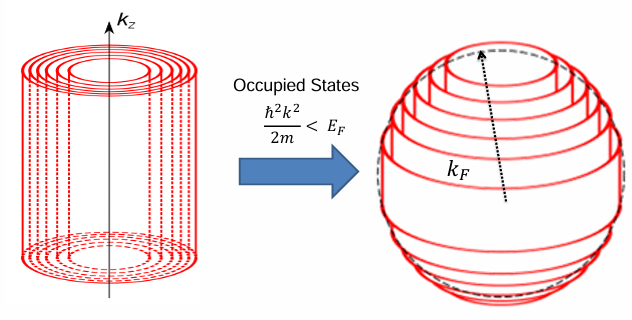
\includegraphics[width=0.8\textwidth]{images/6-Superficie-Fermi/livellilandau.png}
	\caption{I livelli di Landau rappresentano la quantizzazione del moto circolare degli elettroni nel piano per un campo magnetico applicato lungo \(z\).}
	\label{fig:livelli di Landau}
\end{figure}
\begin{figure}[H]
	\centering
	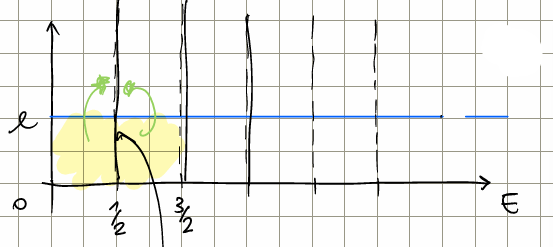
\includegraphics[width=0.6\textwidth]{images/6-Superficie-Fermi/compresslvl.png}
	\caption{Schematizzazione: l'energia contenuta nella corona d'orbite (area evidenziata) viene compressa in un livello discreto, determinato dalla quantizzazione dei livelli di Landau.}
	\label{fig:compress livelli}
\end{figure}


\subsection{Effetto Oscillatorio della Densità di Stati}

Per comprendere il comportamento oscillatorio osservato in molti esperimenti (come l'effetto De Haas--van Alphen) è fondamentale capire come il campo magnetico modifichi la densità di stati elettronici. In particolare, si studiano i casi in cui la densità di stati è calcolata in spazi di dimensioni diverse.

\subsection*{Densità degli Stati in 3 Dimensioni (3D)}

Consideriamo la relazione elementare tra la densità degli stati in \(k\)-space e in \(E\)-space.\\
In 3D il numero di stati in un volume d'elemento \(d\vec{k}\) è proporzionale a:
\[
\rho(E)dE = \rho(k) \, d\vec{k} = \rho(k) \, 4\pi k^2 \, dk\,.
\]
Dato che, per un elettrone libero, l'energia è data da:
\[
E = \frac{\hbar^2 k^2}{2m}\,,
\]
si ottiene, derivando,
\[
dE = \frac{\hbar^2}{m}\, k\, dk \quad \Longrightarrow \quad dk = \frac{m}{\hbar^2\, k}\, dE\,.
\]
Pertanto, sostituendo nell'espressione precedente, la densità degli stati per unità di energia diventa:
\[
\rho_{3D}(E)\, dE = \rho(k) \, 4\pi k^2 \, \frac{m}{\hbar^2\, k}\, dE 
= \rho(k) \, 4\pi k \,\frac{m}{\hbar^2}\, dE
\]
Concludiamo per 
\[\rho(k) = 2\cdot \biggr(\frac{L}{2\pi}\biggr)^3 \]
\[
\rho_{3D}(E) = 2\cdot \biggr(\frac{L}{2\pi}\biggr)^3 \cdot \, 4\pi \frac{m}{\hbar^2}\cdot \sqrt{\frac{2m}{\hbar^2}}\cdot \sqrt{E} = \frac{L^3}{2\pi^2}\cdot \biggr(\frac{2m}{\hbar}\biggr)^\frac{3}{2}\cdot \sqrt{E}\propto \sqrt{E}\,,
\]
ovvero la densità degli stati in 3D cresce come la radice quadrata dell'energia.
\subsection*{Densità degli Stati in 2 Dimensioni (2D)}

In 2D, il numero di stati in un elemento di area nel \(k\)-space è dato da:
\[
\rho_{2D}(E)dE = \rho(k) \, d\vec{k} = \rho(k)\, 2\pi k\, dk\,.
\]
Usiamo nuovamente la relazione energetica per un elettrone libero,
\[
E = \frac{\hbar^2 k^2}{2m} \quad \Longrightarrow \quad dk = \frac{m}{\hbar^2\, k}\,dE\,.
\]
Sostituendo:
\[
\rho_{2D}(E)\, dE = \rho(k)\, 2\pi k\, \frac{m}{\hbar^2\, k}\, dE
= \rho(k)\, 2\pi\, \frac{m}{\hbar^2}\, dE\,.
\]
Inoltre, notando che la densità dei punti in \(k\)-space per un sistema bidimensionale con condizioni periodiche è 
\[\rho(k) = 2\cdot \left(\frac{L}{2\pi}\right)^2\]
risulta che
\[
\rho_{2D}(E) = \frac{mL^2}{\pi\hbar^2}\,,
\]
cioè una quantità costante in funzione dell'energia.  \\
Pertanto, in 2D la densità degli stati è piatta (non dipende da \(E\)).

\subsection*{Densità degli Stati in 1 Dimensione (1D)}

La forma tubolare dei livelli di Landau suggerisce di considerare anche la densità di stati unidimensionale.  
In 1D, il numero di stati in un elemento \(dk\) è dato da:
\[
\rho_{1D}(E)dE = \rho(k)\, dk\,.
\]
Nei sistemi unidimensionali la densità degli stati in \(k\)-space, per condizioni periodiche, è 
\[
\rho(k) = 2\cdot \frac{L}{2\pi}\ = \frac{L}{\pi},.
\]
Per un elettrone libero la relazione energia-momento è:
\[
E = \frac{\hbar^2 k^2}{2m^*}\,,
\]
da cui
\[
dE = \frac{\hbar^2}{m^*}\, k\, dk \quad \Longrightarrow \quad dk = \frac{dE}{\frac{\hbar^2}{m^*}\, k} = \frac{m^*}{\hbar^2 k}\, dE\,.
\]
Sostituendo nell'espressione per la densità degli stati in \(k\)-space,
\[
\rho_{1D}(E)\, dE = \rho(k) \, dk = \frac{L}{\pi} \cdot \frac{m^*}{\hbar^2 k}\, dE\,.
\]
Per eliminare \(k\) in favore dell'energia, usiamo l'equazione
\[
k = \sqrt{\frac{2m^* E}{\hbar^2}}\,,
\]
quindi:
\[
\rho_{1D}(E)\, dE = \frac{L}{\pi}\, \frac{m^*}{\hbar^2\, \sqrt{\frac{2m^* E}{\hbar^2}}}\, dE
=  \frac{L}{\pi}\, \sqrt{\frac{m^*}{2\hbar^2}}\, \frac{dE}{\sqrt{E}}\,.
\]
Così si conclude che
\[
\rho_{1D}(E) \propto \frac{1}{\sqrt{E}}\,.
\]

\section{L'effetto del Campo Magnetico sui Livelli di Landau e sulla Densità degli Stati}

Nel caso in presenza del campo magnetico, gli elettroni sono quantizzati in livelli di Landau.  \\
Per ogni livello (etichettato da \(l\)), la densità di stati risulta modificata e, in particolare, per i livelli di Landau che presentano una natura unidimensionale (movimento libero lungo la direzione del campo) la densità degli stati segue il comportamento:
\[
\rho(E) \propto \frac{1}{\sqrt{E}}\,.
\]
\textbf{Questo significa che ogni volta che l'energia di Fermi \(E_F\) si avvicina al valore corrispondente a uno specifico livello di Landau, la densità degli stati mostra una divergenza (o almeno una grande fluttuazione), determinando il comportamento oscillatorio osservato negli esperimenti.  \\
Infatti, cambiando il campo magnetico (essendo \(\omega_c \propto H\)) la posizione relativa dei livelli di Landau rispetto a \(E_F\) si sposta, provocando una fluttuazione della densità degli stati all'energia di Fermi.}\\\\
Per illustrare questo punto, consideriamo la condizione per cui un elettrone a \(E_F\) occupi il livello \(l\):
\[
E_F = \hbar\omega_c\left(l+\frac{1}{2}\right) 
=\hbar\frac{eH}{m}\left(l+\frac{1}{2}\right)\,.
\]
Da qui si può ricavare:
\[
\frac{E_F}{H} = \frac{\hbar e}{m}\left(l+\frac{1}{2}\right)
\quad \Longrightarrow \quad
\frac{1}{H} = \frac{\hbar e}{mE_F}\left(l+\frac{1}{2}\right)\,.
\]
Indicando con \(A = \frac{\hbar e}{mE_F}\), per \(l=0\) abbiamo:
\[
\frac{1}{H_0} = A\frac{1}{2}\,,
\]
mentre per \(l=1\):
\[
\frac{1}{H_1} = A\frac{3}{2}\,.
\]
Queste relazioni mostrano che la distanza in \(\frac{1}{H}\) (cioè l'intervallo tra i massimi nelle oscillazioni) è determinata dall'area corrispondente alla sezione trasversale della superficie di Fermi e, in generale, varia in modo lineare con \(l+\frac{1}{2}\).\\\\
Plottando \(1/H\) si osserverà quindi una distanza costante tra i massimi, mentre variando il campo magnetico le posizioni relative dei livelli di Landau si spostano.  \\
\textbf{La "larghezza" dei tubi (ovvero delle orbite quantizzate) dipende direttamente dal campo magnetico esterno; all'aumentare di \(H\) i livelli si avvicinano a \(E_F\) e la densità degli stati mostra le divergenze caratteristiche che determinano il comportamento oscillatorio.}

\begin{figure}[H]
    \centering
    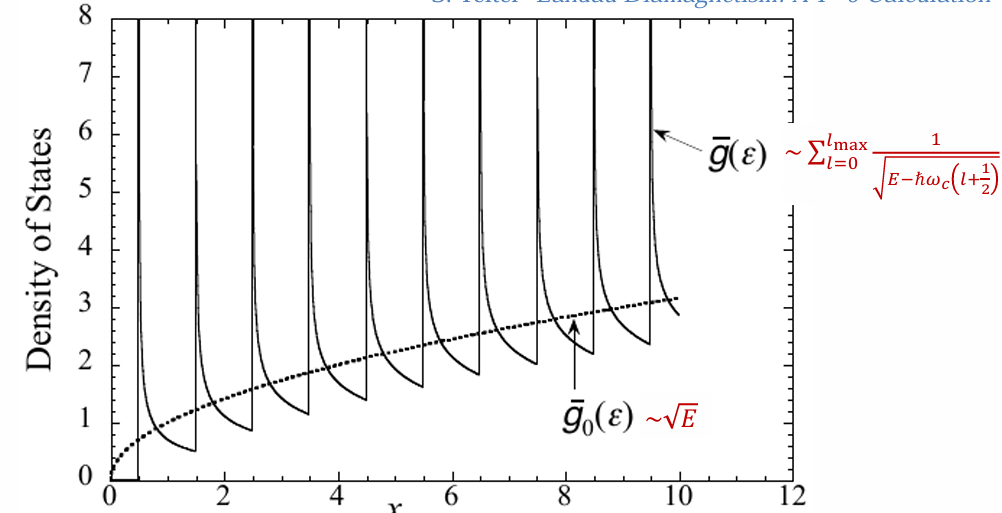
\includegraphics[width=0.9\textwidth]{images/6-Superficie-Fermi/oscillazdos.png}
    \caption{A sinistra, \(g_0(\varepsilon)\) rappresenta la densità degli stati in assenza di campo magnetico, mentre a destra \(g(\varepsilon)\) è quella in presenza del campo magnetico. Le fluttuazioni evidenziano la divergenza quando un livello di Landau si avvicina all'energia di Fermi.}
    \label{fig:oscill-dos}
\end{figure}

\bigskip
\noindent
\textbf{Conclusione:}  
Cambiando \(B\) (o, equivalentemente, \(H\)) si varia il fattore \(\omega_c\) e, di conseguenza, la posizione dei livelli di Landau rispetto a \(E_F\). Questo determina una fluttuazione della densità degli stati all'energia di Fermi, che si manifesta sperimentalmente come un comportamento oscillatorio delle proprietà magnetiche (ad es. oscillazioni in \(\frac{1}{H}\) della suscettività) e nella conduttività.  
In altre parole, la larghezza e la posizione dei "tubi" (orbite quantizzate) dipendono dal campo magnetico esterno: all'aumentare di \(H\) esse si spostano, toccando periodicamente la sfera di Fermi e generando l'oscillazione osservata.  
È importante notare che il "tubo" può intersecare la superficie di Fermi in modi differenti, dando luogo a forme particolari (come ad esempio configurazioni a "clessidra") che forniscono ulteriori informazioni sulla geometria della superficie di Fermi.




\section{Struttura delle bande}
\subsection{Metalli monovalenti}
Hanno la superficie di Fermi più semplice e si dividono in \textbf{metalli nobili} e \textbf{metalli alcalini}. Entrambi hanno un elettrone nella banda di valenza ma la loro struttura elettronica è differente.\\\\

 
 
\subsubsection{Metalli alcalini}
\textbf{I metalli alcalini} hanno la particolarità che le proprietà ottiche e di conduzione rispecchiano perfettamente il modello di Drude-Sommerfeld. Questo perchè i loro elettroni si comportano quasi come elettroni liberi (sfera di Fermi non perfetta per le perturbazioni al secondo ordine), infatti la loro banda di conduzione è formata dagli orbitali s del metallo, che si sovrappongono e creano una banda larga con una densità elettronica relativamente bassa, l'assenza di altri elettroni di valenza implica che la banda di conduzione è poco riempita e i metalli alcalini risultano essere quindi dei eccellenti conduttori.\\\\
La loro superficie di Fermi è una sfera ben contenuta nella prima zona di Brillouin, calcoliamo il raggio della sfera di Fermi che sarà dato da:
\begin{equation}
    \frac{k_F^3}{3\pi^2} = n = \frac{2}{a^3} \implies k_f = \left( \frac{3}{4\pi}\right)^{\frac{1}{3}} \left( \frac{2\pi}{a}\right) = 0,620 \left( \frac{2\pi}{a}\right) 
    \label{eqn:kappaf}
\end{equation}
che proviene dalla relazione tra $k_F$ è la densità di elettroni $n$. La distanza più breve dal centro della zona ad una delle facce (Figura \ref{fig:bcc-met-alc}) è:
\begin{equation} 
    \Gamma N = \frac{2\pi}{a} \sqrt{\left( \frac{1}{2}\right)^2 + \left( \frac{1}{2}\right)^2 + 0^2} = 0,707 \left( \frac{2\pi}{a}\right)
    \label{eqn:gamma-N}
\end{equation}
\begin{figure}
    \centering
    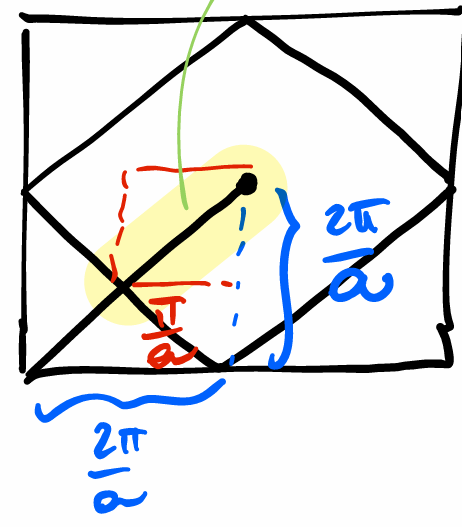
\includegraphics[width=0.2\textwidth]{images/6-Superficie-Fermi/bccmetallialk.png}
    \caption{in (\ref{eqn:gamma-N}) ho calcolato il segmento evidenziato}
    \label{fig:bcc-met-alc}
\end{figure} 

Quindi la sfera di Fermi dell'elettrone libero è interamente contenuta nella prima zona di Brillouin.\\\\
Andando a osservare il grafico in Figura \ref{fig:en-met-alc} vediamo anche che il punto in cui la perturbazione che genera il gap nelle bande è lontana dalla sfera di Fermi, questa è un'altra delle prove a favore del fatto che si comporta come un elettrone libero e questo è perché le proprietà dei metalli, come la conduttività, dipendono dagli elettroni sulla sfera di Fermi, bisgonerebbe andare al secondo ordine per vederne gli effetti. 
\begin{figure}
    \centering
    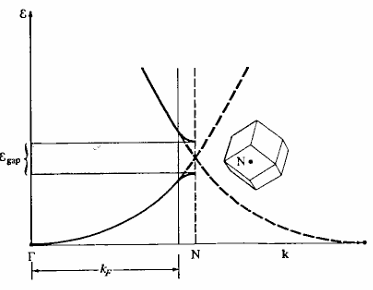
\includegraphics[width=0.7\textwidth]{images/6-Superficie-Fermi/enmetalc.png}
    \caption{}
    \label{fig:en-met-alc}
\end{figure} 

Poi misurando la superficie di Fermi tramite l'effetto di De Haas-van Alphen si conferma sperimentalmente la sfericità della sfera di Fermi in quanto si possono studiare le differenze tra una sfera di Fermi perfetta e ciò che si è ottenuto nel caso del metalli alcalini (Figura \ref{fig:sup-Fermi-met-alc} ) e sono frazioni di percentuale, quindi possiamo finalmente affermare che la loro superficie di Fermi è una sfera. 
\begin{figure}
    \centering
    \includegraphics[width=0.6\textwidth]{images/6-Superficie-Fermi/sup-Fermi-met-alc.png}
    \caption{}
    \label{fig:sup-Fermi-met-alc}
\end{figure}

\subsubsection{Metalli nobili}
\textbf{I metalli nobili} sono duttili perché sono degli FCC che si presentano a strati e quindi sono deformabili, sono caratterizzati da una banda di conduzione che è costituita principalmente dagli orbitali s e d, e le interazioni tra queste bande rendono più complessa la struttura elettronica rispetto ai metalli alcalini. \\
La banda s è larga ed è parzialmente piena (quindi conduce) e si sovrappone con la banda d che è piena, ma altamente localizzata (bassa mobilità) e  vicina in energia agli stati s, questo permette loro di ibridarsi in degli stati ibridi \textbf{sd} che modificano la dispersione (la forma della banda s). Quindi gli stati d:
\begin{itemize}
    \item non partecipano direttamente alla conduzione, ma la influenzano generando questi stati ibridi $sd$ che quando vengono eccitati (assorbimento) permettono più transizioni e quindi modificano la densità degli stati.
    \item gli stati ibridi aumentando la massa efficace degli elettroni di conduzione, questo effetto riduce la mobilità degli elettroni e, di conseguenza, la conducibilità elettrica.
    \item deformano la dipendenza di $\varepsilon$ dal momento $k$, aumenta la densità degli stati vicino all'energia di Fermi,  creando delle perturbazioni uscenti dalla superficie di Fermi che quando toccano i piani di Bragg generano dei gap, ossia aperture al primo ordine che il modello si Sommerfield non può prevedere.
\end{itemize}  
\begin{figure}
    \centering
    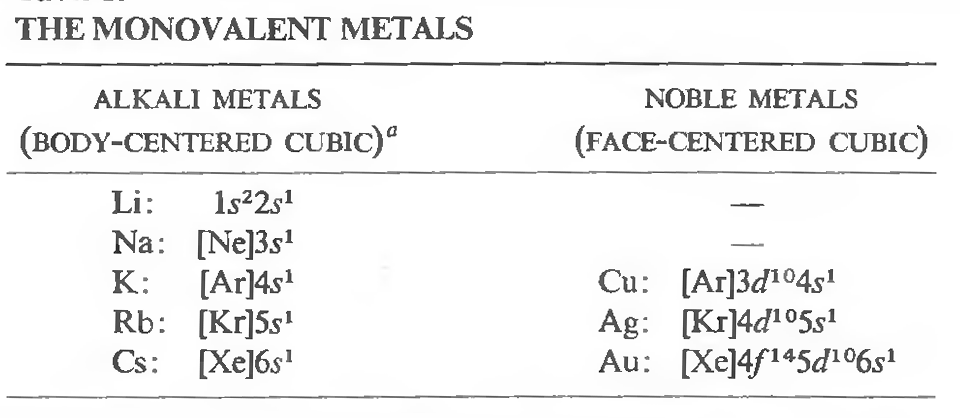
\includegraphics[width=0.9\textwidth]{images/6-Superficie-Fermi/metallimono.png}
    \caption{}
    \label{fig:metalli-monovalenti}
\end{figure} 

Dall'effeto di de Haas-van Alphen si osserva che la loro sfera di Fermi è quasi interamente sferica, però presenta dei "colli" che raggiungono le facce della BZ (Figura \ref{fig:met-nob}). Questo è un effetto di superfici minime e massime è legato alla densità di stati, i tubi in alcuni punti saranno più stretti e in altri sono più larghi, quindi sarò in punti diversi del grafico \ref{fig:oscill-dos}. Per esempio nel caso dell'oro infatti osservo due oscillazioni nella suscettività magnetica e quindi con l'effetto di de Haas-van Alphen quindi posso ottenere una superficie massima ma anche una superficie minima. 
\begin{figure} [H]
    \centering
    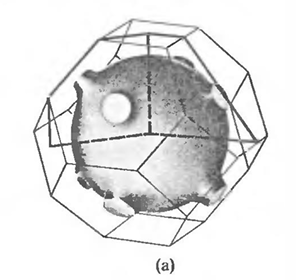
\includegraphics[width=0.3\textwidth]{images/6-Superficie-Fermi/metnob.png}
    \caption{questa è la sfera di Fermi dell'oro}
    \label{fig:met-nob}
\end{figure}


\section*{Proprietà Ottiche dei Metalli Monovalenti}

Il colore di un metallo è determinato dalla dipendenza dalla frequenza della sua riflettività, in quanto alcune frequenze della radiazione incidente vengono riflesse in misura maggiore rispetto ad altre.  
Nel semplice modello a elettrone libero non è possibile riprodurre correttamente le proprietà ottiche poiché, in assenza di collisioni, un elettrone eccitato accelera assorbendo energia e riirraggia la radiazione assorbita, riflettendola quasi completamente, il che non corrisponde alla realtà.  \\
In effetti, è proprio la presenza delle collisioni che fornisce il meccanismo per l'assorbimento dell'energia della radiazione.\\\\
Per elettroni che obbediscono alla legge di Bloch la situazione risulta differente, poiché un processo fortemente dipendente dalla frequenza della radiazione incidente diventa possibile.\\\\
Consideriamo ora un fascio di fotoni avente energia $\hbar\omega$ e momento $\hbar q$ (con il vettore d'onda del fotone $q = 2\pi/\lambda$) che eccita un elettrone da uno stato di energia $\varepsilon$ ad uno stato di energia $\varepsilon'$.  \\
I processi di assorbimento devono soddisfare le seguenti condizioni di conservazione di energia e di momento:

\begin{equation}
    \begin{split}
        \varepsilon' &= \varepsilon + \hbar\omega\,, \\
        k' &= k + q + K\,, \quad \text{con } K \in \text{Reticolo Reciproco (RL)}\,.
    \end{split}
    \label{eqn:con-en-mom}
\end{equation}

Qui si nota che il \textbf{momento cristallino} $k$ non viene conservato nel senso stretto, ma è definito modulo un vettore del reticolo reciproco, per cui
\[
k' = k \pm K\,.
\]
Questo fatto deriva dal potenziale periodico del reticolo, che introduce una perturbazione nello spazio e modifica l'operatore traslazionale collegato al momento.\\
Il meccanismo per il trasferimento di energia $\hbar\omega$ implica che l'elettrone debba passare da una banda ad un'altra (transizioni interbanda), poiché la componente di momento $q$ del fotone è molto più piccola rispetto al valore tipico del vettore d'onda degli elettroni (tipicamente $q \ll k_F$, dove $k_F$ è il raggio della sfera di Fermi).  \\
Pertanto, una transizione interbanda si verifica quando lo stato iniziale si trova al di sotto dell'energia di Fermi e lo stato finale al di sopra, e la frequenza che consente questo salto energetico è detta \textbf{frequenza di soglia}.\\\\
Nei metalli alcalini la banda completamente piena giace ben al di sotto della banda di conduzione.  
Così, l'eccitazione verso la banda di conduzione stabilisce la frequenza di soglia e, mediante un'analisi dettagliata (vedi Figura \ref{fig:trans-banda}), si ottiene la relazione

\[
\hbar\omega = \frac{\hbar^2}{2m}\,(2k_0 - k_F)^2 - \frac{\hbar^2}{2m}\, k_F^2\,,
\]
dove $k_0$ è la distanza (calcolata, ad esempio, lungo la direzione $\Gamma N$ come visto in precedenti analisi) e, sperimentalmente, si trova che $k_F \approx 0,877\, k_0$.  
Da questa relazione si ottiene:
\[
\hbar\omega \approx 0,64\, \varepsilon_F\,,
\]
con $\varepsilon_F$ che indica l'energia di Fermi.

\begin{figure}[H]
    \centering
    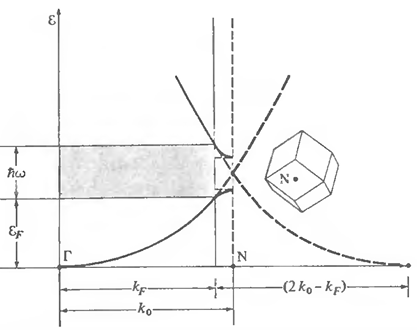
\includegraphics[width=0.6\textwidth]{images/6-Superficie-Fermi/transbanda.png}
    \caption{Schema delle transizioni interbanda in un metallo alcalino.}
    \label{fig:trans-banda}
\end{figure}
\begin{figure}[H]
    \centering
    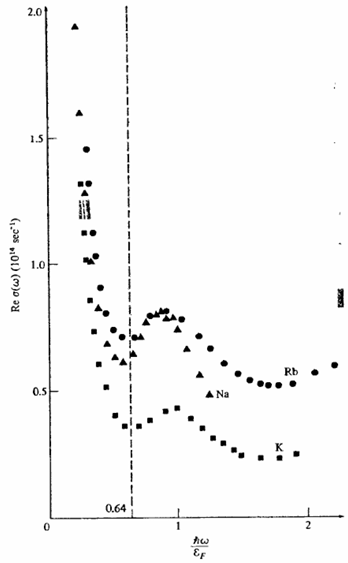
\includegraphics[width=0.6\textwidth]{images/6-Superficie-Fermi/trasm-met-alc.png}
    \caption{Grafico della trasmittanza di alcuni metalli alcalini: si osserva un assorbimento significativo in un intorno di $0,64\,\varepsilon_F$, dove $\varepsilon_F$ è l'energia di Fermi dell'elettrone libero.}
    \label{fig:trasmittanza}
\end{figure}

\section{Metalli Bivalenti e Trivalenti}

\subsection{Metalli Bivalenti}
I metalli divalenti sono quelli la cui struttura elettronica porta ad avere una banda di conduzione parzialmente occupata.  
In Figura \ref{fig:metalli-divalenti} sono riportati alcuni esempi di metalli divalenti.

\begin{figure}[H]
    \centering
    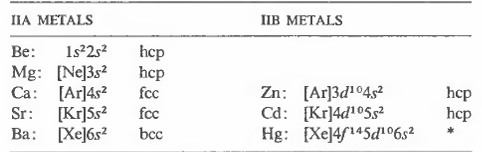
\includegraphics[width=0.7\textwidth]{images/6-Superficie-Fermi/metallidiv.png}
    \caption{Esempi di metalli divalenti.}
    \label{fig:metalli-divalenti}
\end{figure}

\subsection{Metalli Trivalenti}
Tra i metalli trivalenti il caso più semplice è rappresentato dall'alluminio.  
Nel caso dell'alluminio, la prima zona di Brillouin è completamente piena e contiene due elettroni per atomo; il terzo elettrone, invece, si distribuisce nelle seconde e terze zone.  
Si consideri la seguente analisi:

\[
n_e^{II} + n_e^{III} = \frac{n}{3}\,,
\]
dove $n$ è la densità complessiva di elettroni liberi e la suddivisione per 3 deriva dal fatto che, mediamente, vi è un elettrone per cella elementare in eccesso oltre a quelli che occupano la prima zona.  
Inoltre, considerando che in ciascuna zona sono ammessi al massimo due elettroni (degenerazione per spin), si ha:
\[
n_e^{II} + n_h^{II} = 2 \left(\frac{n}{3}\right)\,.
\]
Sottraendo queste due relazioni si ottiene:
\[
n_e^{III} - n_h^{II} = -\frac{n}{3}\,.
\]
Questo risultato indica che, dal punto di vista della conduzione, l'alluminio trasporta una lacuna per atomo.
